\documentclass[11pt]{article}
\usepackage[a4paper,margin=1.9cm]{geometry}
\usepackage[T1]{fontenc}
\usepackage{textcomp}
\usepackage{amsmath,amssymb}
\usepackage{enumitem}
\usepackage{tikz}
\usetikzlibrary{calc,arrows.meta,patterns,decorations.pathmorphing}
\usepackage{xcolor}
\usepackage{multicol}
\usepackage{parskip}
\usepackage{lmodern}
\renewcommand{\familydefault}{\sfdefault}

\definecolor{unalblue}{RGB}{31,73,124}

\newlist{opciones}{enumerate}{1}
\setlist[opciones]{label=(\alph*),itemsep=1pt,topsep=2pt,leftmargin=1.8em,font=\normalfont}

\newcommand{\vect}[2]{\begin{pmatrix}#1\\#2\end{pmatrix}}
\newcommand{\vectiii}[3]{\begin{pmatrix}#1\\#2\\#3\end{pmatrix}}

\newcommand{\examheader}{%
  \noindent
  \begin{minipage}[t]{0.62\linewidth}
    {\bfseries\large C\'alculo en Varias Variables --- Parcial 1}\\
    {\small 13 de marzo de 2023}\\
    {\small Escuela de Matem\'aticas, Universidad Nacional de Colombia, Sede Medell\'in.}
  \end{minipage}%
  \hfill
  \begin{minipage}[t]{0.33\linewidth}
    \raggedleft\small
    Nombre: \rule{2.8cm}{0.4pt}\\[4pt]
    C\'edula: \rule{2.8cm}{0.4pt}
  \end{minipage}\\[4pt]
  \rule{\linewidth}{0.6pt}
}
\newcommand{\examfooter}{%
  \vfill
  \rule{\linewidth}{0.4pt}\\[1pt]
  {\scriptsize\textit{Transcripci\'on digital --- MathUNAL}\hfill\textcolor{unalblue}{\textbf{\thepage}}}
}
\pagestyle{empty}

\begin{document}

\examheader

\textbf{Instrucciones:} La duraci\'on del examen es de 1 hora y 45 minutos. Antes de empezar verifique que su examen est\'e completo y que sus datos sean correctos. No desengrape su examen ni a\~nada otras grapas. Use los espacios asignados para resolver cada pregunta. \textbf{No} est\'a permitido: hacer preguntas, usar calculadoras, sacar hojas en blanco, ni tomar apuntes en hojas diferentes a las del examen. Tampoco se permite el uso de celulares, ni smartphones, ni tabletas digitales.

\bigskip

\textit{En las preguntas 1 a 4 no se tendr\'a en cuenta el procedimiento.}

\bigskip
\noindent\textbf{1.} (10\,\%) Sea $f(x,y)=2y+2e^{y^2x}$. La derivada direccional de $f$ en el punto $(-1,\sqrt2)$, en la direcci\'on del vector $v=\langle 1,2\rangle$, es:
$$\text{Respuesta:}\ \underline{\hspace{5cm}}$$

\bigskip
\noindent\textbf{2.} (10\,\%) Una ecuaci\'on del plano tangente a la gr\'afica de la funci\'on $g(x,y)=2x-2e^{y^2x}$, en el punto $(1,\sqrt2,g(1,\sqrt2))$, es

\begin{opciones}
  \item $z = -2(1-e^2)x - 4\sqrt2\,e^2y + 8+14e^2$
  \item $z = 2(1-2e^2)x - 4\sqrt2\,e^2y + 10e^2$
  \item $z = 2(1-2e^2)x - 4\sqrt2\,e^2y + 6e^2$
  \item $z = -2(1-e^2)x + 4\sqrt2\,e^2y + 8-2e^2$
\end{opciones}

\bigskip
\noindent\textbf{3.} (10\,\%) Grafique en la cuadr\'icula y sombree el dominio de la funci\'on
$$f(x,y) = \ln(2y-x-2) + \sqrt{2x-y-2}.$$

\begin{center}
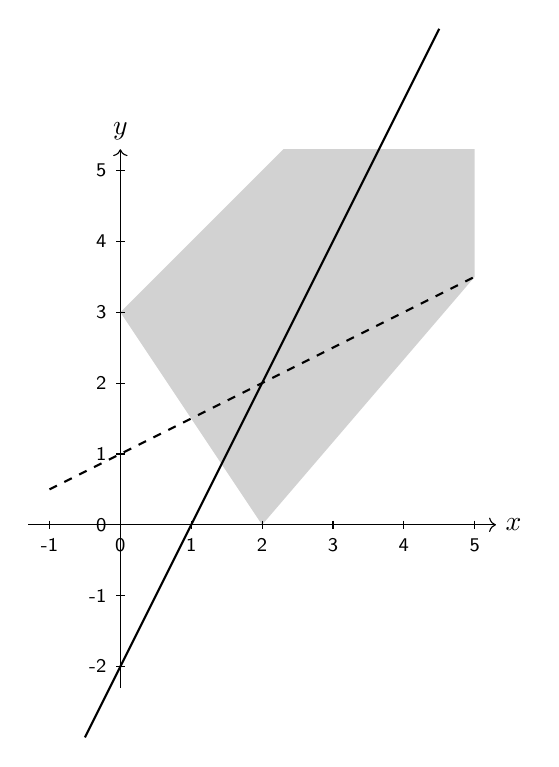
\begin{tikzpicture}[scale=0.9]
  \begin{scope}
    \clip (-1.3,-2.3) rectangle (5.3,5.3);
    \path[use as bounding box] (-1.3,-2.3) rectangle (5.3,5.3);
    % region: y > (x+2)/2  AND  y <= 2x-2
    \fill[gray!35] (2,0) -- (5,3.5) -- (5,8) -- (0,3) -- cycle;
  \end{scope}
  \draw[->] (-1.3,0) -- (5.3,0) node[right]{$x$};
  \draw[->] (0,-2.3) -- (0,5.3) node[above]{$y$};
  \foreach \x in {-1,0,1,2,3,4,5}{\draw (\x,0.06)--(\x,-0.06) node[below,font=\scriptsize]{\x};}
  \foreach \y in {-2,-1,0,1,2,3,4,5}{\draw (0.06,\y)--(-0.06,\y) node[left,font=\scriptsize]{\y};}
  \draw[thick,dashed,domain=-1:5] plot(\x,{\x/2+1});
  \draw[thick,domain=-0.5:4.5] plot(\x,{2*\x-2});
\end{tikzpicture}
\end{center}

\begin{opciones}
  \item[$\bullet$] (3\,\%) El dominio de la funci\'on $\displaystyle h(x,y)=\frac{(x-2)^2}{4-y^2}$ es $D = \left\{(x,y)\in\mathbb{R}^2 \mid y\neq\pm 2\right\}$.
  \item[$\bullet$] (7\,\%) Grafique la curva de nivel de valor $1$ para la funci\'on $\displaystyle h(x,y)=\frac{(x-2)^2}{4-y^2}$.
\end{opciones}

\begin{center}
\begin{tikzpicture}[scale=0.8]
  \draw[->] (-1.3,0) -- (5.3,0) node[right]{$x$};
  \draw[->] (0,-3.3) -- (0,3.3) node[above]{$y$};
  \foreach \x in {-1,0,1,2,3,4,5}{\draw (\x,0.06)--(\x,-0.06) node[below,font=\scriptsize]{\x};}
  \foreach \y in {-3,-2,-1,0,1,2,3}{\draw (0.06,\y)--(-0.06,\y) node[left,font=\scriptsize]{\y};}
  \draw[thick] (2,0) circle (2);
  \fill (2,2) circle (1.5pt);
  \fill (2,-2) circle (1.5pt);
\end{tikzpicture}
\end{center}

\newpage
\examheader
\vspace{2pt}

\textit{En las preguntas 5, 6 y 7 debe realizar el procedimiento justificando cada paso.}

\bigskip
\noindent\textbf{5.} (20\,\%) Halle $f_y(x,y)$ para la funci\'on escalar de dos variables definida por
$$
f(x,y)=
\begin{cases}
\dfrac{x^3+2y^3}{x^2+y^2}, & (x,y)\neq (0,0),\\[6pt]
0, & (x,y)=(0,0).
\end{cases}
$$

\bigskip
\bigskip
\noindent\textbf{6.} (20\,\%) Halle el punto en la superficie $S:\; x^2-2x+y^2+4-z=0$ en el cual el plano tangente a $S$ es paralelo al plano tangente a $x+y^2+z=6$ en el punto $(2,1,3)$.

\vfill
\examfooter
\newpage
\examheader
\vspace{2pt}

\noindent\textbf{7.} (20\,\%) Suponga que la porci\'on de un \'arbol que se puede utilizar para extraer madera es un cilindro circular recto. La altura utilizable del \'arbol aumenta 8 pulgadas por a\~no y el di\'ametro utilizable aumenta 2 pulgadas por a\~no. ¿Qu\'e tan r\'apidamente crece el volumen de madera utilizable cuando la altura utilizable es de 80 pulgadas y el di\'ametro es de 10 pulgadas?
$$\text{Respuesta:}\ \underline{\hspace{6cm}}$$

\vfill
\examfooter

\end{document}
